\documentclass[a4paper,12pt]{article}
\usepackage[top = 2.5cm, bottom = 2.5cm, left = 2.5cm, right = 2.5cm]{geometry}
\usepackage[T1]{fontenc}
\usepackage[utf8]{inputenc}
\usepackage{multirow} 
\usepackage{booktabs} 
\usepackage{graphicx}
\usepackage[spanish]{babel}
\usepackage{setspace}
\setlength{\parindent}{0in}
\usepackage{float}
\usepackage{fancyhdr}
\usepackage{amsmath}
\usepackage{amssymb}
\usepackage{amsthm}
\usepackage[numbers]{natbib}
\newcommand\Mycite[1]{%
	\citeauthor{#1}~[\citeyear{#1}]}
\usepackage{graphicx}
\usepackage{subcaption}
\usepackage{booktabs}
\usepackage{etoolbox}
\usepackage{minibox}
\usepackage{hyperref}
\usepackage{xcolor}
\usepackage[skins]{tcolorbox}
%---------------------------

\newtcolorbox{cajita}[1][]{
	 #1
}

\newenvironment{sol}
{\renewcommand\qedsymbol{$\square$}\begin{proof}[\textbf{Solución.}]}
	{\end{proof}}

\newenvironment{dem}
{\renewcommand\qedsymbol{$\blacksquare$}\begin{proof}[\textbf{Demostración.}]}
	{\end{proof}}

\newtheorem{problema}{Problema}
\newtheorem{definicion}{Definición}
\newtheorem{ejemplo}{Ejemplo}
\newtheorem{teorema}{Teorema}
\newtheorem{corolario}{Corolario}[teorema]
\newtheorem{lema}[teorema]{Lema}
\newtheorem{prop}{Proposición}
\newtheorem*{nota}{\textbf{NOTA}}
\renewcommand\qedsymbol{$\blacksquare$}
\usepackage{svg}
\usepackage{pgfplots}
\pgfplotsset{compat=1.11}

\usepackage{tikz}
\usetikzlibrary{calc}

\usetikzlibrary{patterns}
\usepackage[framemethod=default]{mdframed}
\global\mdfdefinestyle{exampledefault}{%
linecolor=lightgray,linewidth=1pt,%
leftmargin=1cm,rightmargin=1cm,
}




\newenvironment{noter}[1]{%
\mdfsetup{%
frametitle={\tikz\node[fill=white,rectangle,inner sep=0pt,outer sep=0pt]{#1};},
frametitleaboveskip=-0.5\ht\strutbox,
frametitlealignment=\raggedright
}%
\begin{mdframed}[style=exampledefault]
}{\end{mdframed}}
\newcommand{\linea}{\noindent\rule{\textwidth}{3pt}}
\newcommand{\linita}{\noindent\rule{\textwidth}{1pt}}

\AtBeginEnvironment{align}{\setcounter{equation}{0}}
\pagestyle{fancy}

\fancyhf{}









%----------------------------------------------------------
\lhead{\footnotesize Geometría diferencial}
\rhead{\footnotesize  Rudik Roberto Rompich}
\cfoot{\footnotesize \thepage}


%--------------------------

\begin{document}
 \thispagestyle{empty} 
    \begin{tabular}{p{15.5cm}}
    \begin{tabbing}
    \textbf{Universidad del Valle de Guatemala} \\
    Departamento de Matemática\\
    Licenciatura en Matemática Aplicada\\\\
   \textbf{Estudiante:} Rudik Roberto Rompich\\
   \textbf{Correo:}  \href{mailto:rom19857@uvg.edu.gt}{rom19857@uvg.edu.gt}\\
   \textbf{Carné:} 19857
    \end{tabbing}
    \begin{center}
        Geometría diferencial - Catedrático: Alan Reyes\\
        \today
    \end{center}\\
    \hline
    \\
    \end{tabular} 
    \vspace*{0.3cm} 
    \begin{center} 
    {\Large \bf  Tarea
} 
        \vspace{2mm}
    \end{center}
    \vspace{0.4cm}
%--------------------------

\begin{problema}
    
    Sea $\alpha$ una curva de Frenet en $\mathbb{R}^{n}$. Muestre que

$$
\operatorname{det}\left[\alpha^{\prime}, \alpha^{\prime \prime}, \alpha^{\prime \prime \prime}, \ldots, \alpha^{(n)}\right]=\prod_{i=1}^{n-1} \kappa_{i}^{(n-i)} .
$$
    \begin{sol}
        Como $\alpha$ es una curva de Frenet, se cumple la definición, tal que  $$\alpha(\mathrm{s}): I \subseteq \mathbb{R} \rightarrow \mathbb{R}^n$$ una curva regular, parametrizada por longitud de arco, y de clase $C^n$. $\alpha$ es una curva de Frenet si en todo punto $s$, los vectores $\alpha^{\prime}(\mathrm{s}), \alpha^{\prime \prime}(\mathrm{s}), \ldots, \alpha^{(n-1)}(\mathrm{s})$ son linealmente independientes. 
        Además, también se mencion al referencial de Frenet de $\alpha$ se define como $\left\{\mathbf{e}_1, \mathbf{e}_2, \ldots, \mathbf{e}_n\right\}$ y está únicamente determinado por
        \begin{itemize}
            \item $\left\{\mathbf{e}_1, \mathbf{e}_2, \ldots, \mathbf{e}_n\right\}$ es una base ortonormal de $\mathbb{R}^n$.
            \item Para todo $k=1, \ldots, n-1,\left\langle\mathbf{e}_1, \ldots, \mathbf{e}_k\right\rangle=\left\langle\alpha^{\prime}(s), \ldots, \alpha^{(k)}(s)\right\rangle$.
            \item $\left\langle\alpha^{(k)}(s), \mathbf{e}_k\right\rangle>0$, para $k=1, \ldots, n-1$.
        \end{itemize}
        Entonces, por construcción de teorema visto en clase, tenemos que: 
        $$\left(\begin{array}{c}\mathbf{e}_1^{\prime} \\ \mathbf{e}_2^{\prime} \\ \vdots \\ \vdots \\ \mathbf{e}_{n-1}^{\prime} \\ \mathbf{e}_n^{\prime}\end{array}\right)=\left(\begin{array}{cccccc}0 & \kappa_1 & 0 & 0 & \cdots & 0 \\ -\kappa_1 & 0 & \kappa_2 & 0 & \ddots & \vdots \\ 0 & -\kappa_2 & 0 & \kappa_3 & \ddots & 0 \\ 0 & 0 & \ddots & \ddots & \kappa_{n-2} & 0 \\ \vdots & \ddots & 0 & -\kappa_{n-2} & \cdots & \kappa_{n-1} \\ 0 & \cdots & 0 & 0 & -\kappa_{n-1} & 0\end{array}\right)\left(\begin{array}{c}\mathbf{e}_1 \\ \mathbf{e}_2 \\ \vdots \\ \vdots \\ \mathbf{e}_{n-1} \\ \mathbf{e}_n\end{array}\right), \forall s$$

        Es decir que esencialmente, 
        $$\alpha^{(k)} =\kappa_1\kappa_2\kappa_3\cdots\kappa_{k-1}\mathbf{e}_k$$
        Entonces, 
        \begin{align*}
            \det \left[\alpha^{\prime}, \alpha^{\prime \prime}, \alpha^{\prime \prime \prime}, \ldots, \alpha^{(n)}\right]&=\det \left[\alpha^{\prime}, \alpha^{\prime \prime}, \alpha^{\prime \prime \prime}, \ldots, \alpha^{(n)}\right]\\
            &= \det \left[\mathbf{e}_1,\kappa_1\mathbf{e}_2, \kappa_1\kappa_2\mathbf{e}_3, \ldots, \kappa_1\kappa_2\kappa_3\cdots\kappa_{k-1}\mathbf{e}_k\right]\\
            &= \kappa_1^{n-1} \cdot \kappa_2^{n-2} \cdot \kappa_3^{n-3} \cdots \kappa_{n-2}^2 \cdot \kappa_{n-1}\\
            &=\prod_{i=1}^{n-1} \kappa_{i}^{(n-i)}
        \end{align*}
    \end{sol}


\end{problema}


\begin{problema}
    Construir una curva, no planar, de clase $C^{\infty}$ en $\mathbb{R}^{3}$, que sea una curva de Frenet, excepto en un único punto, y que fuera de ese punto, satisface $\tau \equiv 0$.
    \begin{sol}
        En clase, se vio que la hélice es una curva de Frenet en $\mathbf{R}^3$. Considerando que el círculo es un caso especial de la hélice en $\mathbf{R}^3$, considérese las siguientes curvas
        \begin{align*}
            \alpha_1(s) &= \left(\cos \left(\frac{1}{t}\right), \sin\left(\frac{1}{t}\right),0 \right)\\
            \alpha_2(s) &= \left(0, \cos \left(\frac{1}{t}\right), \sin\left(\frac{1}{t}\right)\right)\\
        \end{align*}
        Estás curvas son de Frenet en todo punto, excepto en $t=0$. Sin embargo, si hacemos una unión de las curvas, 
        $$\alpha_1(s)\cup \alpha_2(s)$$
        Tenemos una curva no planar, de clase $C^\infty$, que es de Frenet, excepto en un punto y que $\tau\equiv 0$. 
    \end{sol}
\end{problema}

\begin{problema} 
    Sea
    \begin{enumerate}
        \item Sea $\alpha:[0, L] \rightarrow \mathbb{R}^{2}$ una curva plana, cerrada y simple, parametrizada por longitud de arco. Suponga que $0 \leq \kappa(s) \leq c$, $\forall s \in[0, L]$, para alguna constante $c>0$. Probar que $L \geq \frac{2 \pi}{c}$.
        \begin{sol}
            Por definición de índice de rotación para curvas cerradas y como es simple $I=1$,
            $$\int_0^L \kappa(s) ds=2\pi $$
            Por hipótesis, tenemos que $0 \leq \kappa(s) \leq c$, entonces: 
            $$\int_0^L \kappa(s) ds\leq c\int_0^L ds=cL$$
            Por lo tanto, 
            $$2\pi \leq cL\implies L \geq \frac{2 \pi}{c}$$
        \end{sol}
        \item Si reemplazamos la hipótesis de $\alpha$ ser simple por $\alpha$ tiene índice de rotación $I$, probar que $L \geq \frac{2 \pi I}{c}$.
        \begin{sol}
            La prueba es análoga, 
            $$\int_0^L \kappa(s) ds=2\pi I  $$
            Por hipótesis, tenemos que $0 \leq \kappa(s) \leq c$, entonces: 
            $$\int_0^L \kappa(s) ds\leq c\int_0^L ds=cL$$
            Por lo tanto, 
            $$2\pi I \leq cL\implies L \geq \frac{2 \pi I}{c}$$
        \end{sol}
    \end{enumerate}
\end{problema}

\begin{problema}
    Sea $\alpha:[0, L] \rightarrow \mathbb{R}^{2}$ una curva plana, cerrada y convexa, orientada de forma positiva. La curva

    $$
    \beta(s)=\alpha(s)-r \mathbf{n}(s),
    $$
    
    donde $r>0$ es una constante positiva y $\mathbf{n}(s)$ es el vector normal de $\alpha$ en $s$, se llama una curva paralela a $\alpha$. Muestre que
    \begin{enumerate}
        \item $\ell(\beta)=\ell(\alpha)+2 \pi r$
        \begin{sol}
            Sea 
            \begin{align*}
                \ell(\beta) &= \int_0^L |\beta'(s)|ds\\
                &= \int_0^L |\alpha'(s)-r \mathbf{n}'(s)|ds\\
                &= \int_0^L |\alpha'(s)-r\left(-\kappa \mathbf{T}(s)+\tau\mathbf{B}(s)\right)|ds\\
                &= \int_0^L \left|\alpha'(s)-r\left(-\kappa \left(\frac{\alpha'(s)}{|\alpha'(s)|}\right)+\tau\mathbf{B}(s)\right)\right|ds
                \intertext{Como $\alpha$ es plana, $\tau=0$. Además, considerando la definición de longitud de arco, $s$ es el parámetro natural de $\alpha$, tal que $|\alpha'(s)|=|\mathbf{T}(s)|=1$.}
                &= \int_0^L \left|\alpha'(s)-r\left(-\kappa \left(\frac{\alpha'(s)}{1}\right)+0\mathbf{B}(s)\right)\right|ds\\
                &= \int_0^L \left|\alpha'(s)+r\kappa\alpha'(s) \right|ds\\
                &= \int_0^L |\alpha'(s)|\left|1+r\kappa\right|ds\\
                &= \int_0^L \left|1+r\kappa\right|ds
                \intertext{Como $r>1$ y la curva es orientada positivamente,}
                &= \int_0^L(1+r\kappa)ds\\
                &= L + r\int_0^L\kappa ds
                \intertext{Por definición de índice de rotación para curvas cerradas y simples, y cosiderando $L=\ell(\alpha)$}
                &= \ell(\alpha) + 2\pi r
            \end{align*}
              
            
        \end{sol}
        \item $A(\beta)=A(\alpha)+r L+\pi r^{2}$.
        \begin{sol}
            Por el inciso anterior, sea $\ell(\beta)=\ell(\alpha)+2\pi t$, entonces el área entre las dos curvas paralelas lo podemos definir como:
            \begin{align*}
                A(\beta) - A(\alpha) &= \int_0^r \ell(\beta)dt\\
                &= \int_0^r \ell(\alpha)+2\pi tdt\\
                &=\ell(\alpha)r+\pi r^2\\
                &=Lr+\pi r^2
            \end{align*}
            Despejando, obtenemos: 
            $$A(\beta)=A(\alpha)+r L+\pi r^{2}$$
        \end{sol}
        \item $\kappa_{\beta}(s)=\frac{\kappa_{\alpha}(s)}{1+r \kappa_{\alpha}(s)}$.
        \begin{sol}
            Sea
            \begin{align*}
                \kappa_{\beta}(s) &= \frac{\left|\beta' \times \beta''\right|}{|\beta'|^3}
            \end{align*}
            En donde, por el inciso 1, 
            \begin{align*}
                \beta' &= \alpha'(s)(1+r\kappa_\alpha) = \mathbf{T}(s)(1+r\kappa_\alpha)\\
                \beta'' &=  \mathbf{T}'(s)+r\left(\kappa_\alpha'\mathbf{T}(s)+\kappa_\alpha \mathbf{T}'(s)\right)\\
                &=(1+r\kappa_\alpha)\mathbf{T}'(s)+r\kappa_\alpha'\mathbf{T}(s)
            \end{align*}
            Entonces: 
            \begin{align*}
                \kappa_{\beta}(s) &= \frac{\left|\beta' \times \beta''\right|}{|\beta'|^3}\\
                &= \frac{\left|(\mathbf{T}(s)(1+r\kappa_\alpha)) \times ((1+r\kappa_\alpha)\mathbf{T}'(s)+r\kappa_\alpha'\mathbf{T}(s))\right|}{|\mathbf{T}(s)(1+r\kappa_\alpha)|^3}\\
                &= \frac{\left| (1+r\kappa_\alpha)^2\mathbf{T}(s)\times \mathbf{T}'(s)
                +(1+r\kappa_\alpha)r\kappa_\alpha'\mathbf{T}(s)\times \mathbf{T}(s)\right|}{|\mathbf{T}(s)(1+r\kappa_\alpha)|^3}
                \intertext{Se conoce $\mathbf{T}(s)\times \mathbf{T}(s)=0$ y $\mathbf{T}(s)=1$,}
                &= \frac{ (1+r\kappa_\alpha)^2\left|\mathbf{T}(s)\times \mathbf{T}'(s)\right|}{(1+r\kappa_\alpha)^3}\\
                &= \frac{\kappa_\alpha}{1+r\kappa_\alpha}
            \end{align*}
        \end{sol}
    \end{enumerate}
    
\end{problema}

\begin{problema}
    Sea $C:[0, L] \rightarrow \mathbb{R}^{2}$ una curva plana, cerrada, orientada positivamente, con $\kappa>0$. Asuma que $C$ posee al menos un punto de auto-intersección p. 
    \begin{figure}[H]
        \centering
        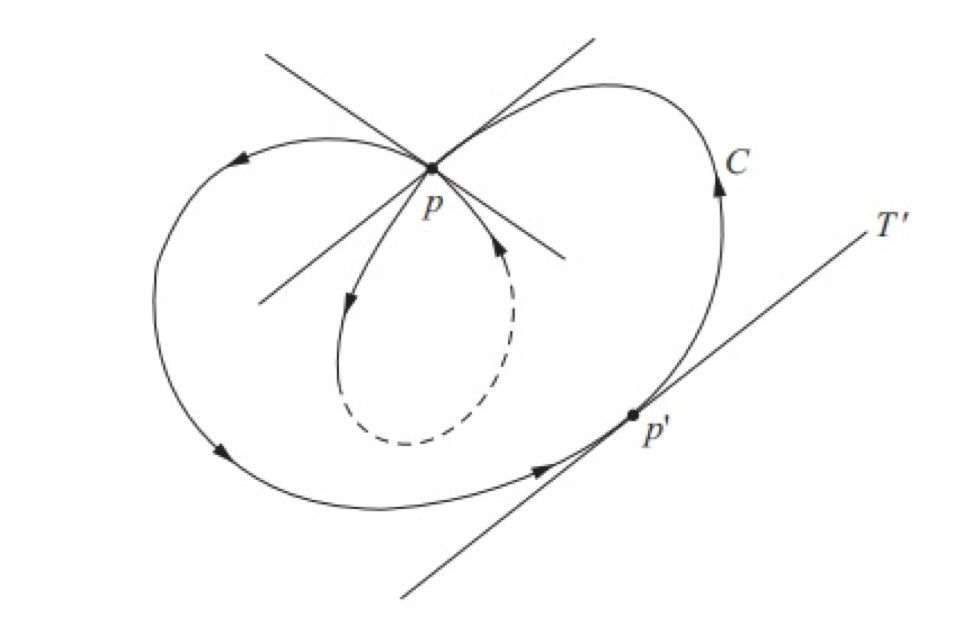
\includegraphics[scale=0.5]{imagenes/im5.png}
    \end{figure}
    
    Demostrar que

    \begin{enumerate}
        \item $C$ posee al menos una tangente doble.
            \begin{sol}
                Usando el Teorema de Fabricius-Bjerre, 
                sabemos
                \begin{align*}
                    N^+ &=N^- +D +\frac{1}{2}W
                \end{align*}
                Como $\kappa>0$, entonces $W=0$. Por hipótesis, $D\geq 1$.  Considerando también que $N^-\geq 0$. Nos permite asegurar que $ N^+\geq 1$. Por lo tanto $C$ al menos posee una tangente doble. 
            \end{sol}
        \item Existe un punto $\mathbf{p}^{\prime}$ cuya tangente a $C$ en $\mathbf{p}^{\prime}$ es paralela a la tangente a $C$ en $\mathbf{p}$. 
        \begin{sol}
            Inmediatamente usando la interpretación del teorema del valor medio de Cauchy. Nótese que las dos tangentes en $p$ son secantes de $C$. Entonces, sea $f(t)$ la longitud de arco de $C$ en $[0,L]$ y sea $g(t)$ el área encerrada de $C$. Como la curva es cerrada $f(a)=f(b)=0$. Por lo tanto, 
            \begin{align*}
                f'(p') &= \frac{f(b)-f(a)}{g(b)-g(a)}g'(p')\\
                      &= \frac{0}{g(b)-g(a)}g'(p')\\
                      &= 0
            \end{align*}
            Es decir, que la tangente en $p'$ es paralela a una de las secantes (que también es tangente) en $p$. 
        \end{sol}
        \item El ángulo de rotación de la tangente en el arco positivo de $C$ dado por $\mathbf{p p}^{\prime} \mathbf{p}$ es mayor a $\pi$.
        \begin{sol}
            Sea $\theta$ el ángulo pequeño entre las dos tangentes de $p$ y $\phi$ el más grande. Entonces nótese que al dar una rotación por $\mathbf{p p}^{\prime} \mathbf{p}$ Se cumple que $$\theta+\phi +\theta = (\theta+\phi)+\theta = \pi +\theta >\pi $$  
        \end{sol}
        \item  El índice de rotación de $C$ es $I \geq 2$.
        \begin{sol}
            Ya que tiene como mínimo una autointersección, entonces el índice es mayor a 1. Por lo tanto, $I\geq 2$. 
        \end{sol}
    \end{enumerate}

\end{problema}

\begin{problema}
    Hallar todos los vértices de la elipse $\gamma(t)=(p \cos t, q \sin t)$, cuando $p \neq q$ (aquí, $p, q>0)$.
    \begin{sol}
        Para este problema, usamos el procedimiento usado en la demostración del teorema de los cuatro vértices. 
        Primero, consideramos la ecuación de la curvatura de una parametrización definido como: 
        \begin{align*}
            \kappa &= \frac{|x'y''-y'x''|}{(x'^2+y'^2)^{3/2}}\\
            &= \frac{|(-p\sin t)(-q\sin t)-(q\cos t)(-p\cos t)|}{((-p\sin t)^2+(q\cos t)^2)^{3/2}}\\
            &= \frac{|pq\sin^2 t+pq \cos^2 t|}{(p^2\sin^2 t+q^2\cos^2 t)^{3/2}}\\
            &= \frac{|pq|}{(p^2\sin^2 t+q^2\cos^2 t)^{3/2}}\\
            &= \frac{pq}{(p^2\sin^2 t+q^2\cos^2 t)^{3/2}}
        \end{align*}
        Para hallar los vértices, debemos encontrar las máximos y mínimos de la curvatura, es decir $\kappa'=0$. Para esto, derivamos la expresión: 
        \begin{align*}
            \kappa' &= \frac{f'g- fg'}{g^2}\\
                    &= pq\left(\frac{0-3\left(p^2-q^2\right)\sin t \cos t \sqrt{p^2 \sin^2 t + q^2 \cos^2 t}}{(p^2\sin^2 t+q^2\cos^2 t)^3}\right)\\
                    &= \frac{3pq\left(q^2-p^2\right)\sin t \cos t }{(p^2\sin^2 t+q^2\cos^2 t)^{5/2}}\\
        \end{align*}
        Igualamos a cero la expresión anterior, tal que: 
        \begin{align*}
            \frac{3pq\left(q^2-p^2\right)\sin t \cos t }{(p^2\sin^2 t+q^2\cos^2 t)^{5/2}} &= 0\\
            \sin t \cos t &= 0
        \end{align*}
        Como ya sabemos que $t\in [0,2\pi]$, tenemos que 
        \begin{itemize}
            \item $\sin t = 0$, cuando $t=0,\pi,2\pi$
            \item $\cos t = 0$, cuando $t=\frac{\pi}{2},\frac{3\pi}{2}$
        \end{itemize}
        Con esto, evaluamos en la parametrización original, tal que los vértices son: 
        \begin{itemize}
            \item $t=0,\pi,2\pi$:
            \begin{itemize}
                \item $(p \cos 0, q \sin 0)=(p,0)$
                \item $(p \cos \pi, q \sin \pi)=(-p,0)$
                \item $(p \cos 2\pi, q \sin 2\pi)=(p,0)$
            \end{itemize}
            \item $t=\pi/2,3\pi/2$:
            \begin{itemize}
                \item $(p \cos \pi/2, q \sin \pi/2)=(0,q)$
                \item $(p \cos 3\pi/2, q \sin 3\pi/2)=(0,-q)$
            \end{itemize}
        \end{itemize}
    \end{sol}
\end{problema}
%---------------------------
%\bibliographystyle{apa}
%\bibliography{referencias.bib}

\end{document}